\documentclass[12pt,a4paper]{article}
\usepackage[margin=2.5cm]{geometry}
\usepackage{fontspec,polyglossia}
\setmainlanguage[numerals=maghrib]{arabic}
\setotherlanguage{english}
% Shared Arabic font families for XeLaTeX (Amiri with explicit bold/italic).
\defaultfontfeatures{Ligatures=TeX}
\newfontfamily\arabicfont[
  Script=Arabic,
  Language=Arabic,
  Scale=1.05,
  BoldFont={Amiri Bold},
  ItalicFont={Amiri Italic},
  BoldItalicFont={Amiri Bold Italic}
]{Amiri}
\newfontfamily\arabicfontsf[
  Script=Arabic,
  Language=Arabic,
  Scale=1.05,
  BoldFont={Amiri Bold},
  ItalicFont={Amiri Italic},
  BoldItalicFont={Amiri Bold Italic}
]{Amiri}
\newfontfamily\arabicfonttt[
  Script=Arabic,
  Language=Arabic,
  Scale=0.95,
  BoldFont={Amiri Bold}
]{Amiri}

\usepackage{amsmath,amssymb,amsthm,algorithm,algpseudocode,graphicx,hyperref}
\graphicspath{{../../figures/}}
\title{\textbf{VR-DA-SFCN: نيوتن تكعيبي خالٍ من السرج مخفَّض التباين}\\
\large للمجاميع المنتهية}
\author{الورقة 2 من 6 --- مجموعة التحسين العددي}
\date{سبتمبر 2026}
\begin{document}
\maketitle
\begin{abstract}
نرفع \textenglish{DA-SFCN} إلى $f=\frac1N\sum f_i$ بتغذية النواة التكعيبية
الكريلوفية بمتغيرات تحكم \textenglish{SVRG} على التدرّج وجداء الهيسيان--متجه
معًا. تُحدَّث لقطة $\tilde x$ كل $T$ خطوات، وبين اللقطات تعطي دفعة $B$
\[
g^{\mathrm{vr}}=\nabla f_B(x)-\nabla f_B(\tilde x)+\nabla f(\tilde x).
\]
يُورَث المعدل العالمي $O(k^{-2/3})$ بالتوقع متى كانت فجوة اللقطة من رتبة
$\|\nabla f\|$. على مجموع 30 تربيعية غير محدبة يتفوق الأوراكل الكامل في
عدد التكرارات (8 مقابل 60) كما تتوقع النظرية، بينما يبقى \textenglish{VR-DA-SFCN}
الخيار العملي عندما يجعل $N$ الجداء الكامل باهظًا. وعلى اللوجستي تبلغ
$\|\nabla f\|\approx 4.7\times 10^{-14}$.
\end{abstract}

\section{الدافع}
جداء هيسيان--متجه كامل يكلّف $N$ جداءات محلية. التكعيب العشوائي يستبدل ذلك
بدفعة فيُدخل تباينًا يفسد اختبار \textenglish{ARC} وتعامد \textenglish{Lanczos}.
تخفيض التباين ليس تسريعًا اختياريًا بل شرط استقرار إحصائي.

\section{الخوارزمية}
كل $T$ خطوات نعيد اللقطة والتدرّج الكامل. وفي ما بينها نأخذ دفعة ونبني
$g^{\mathrm{vr}}$ و$H^{\mathrm{vr}}v$ ثم ننفّذ خطوة \textenglish{DA-SFCN}
واحدة بالجدولة اللوغاريتمية والنموذج $|T|$.

\section{مخطط التحليل}
الفرق $g^{\mathrm{vr}}-g$ من رتبة $\|x-\tilde x\|$ بليبشتزية الهيسيان.
فإذا أُنعشت اللقطة كلما تجاوزت الفجوة مضاعفًا من $\|g\|$ صار اضطراب النموذج
من رتبة $\|g\|$ وامتصّه $M_k$. وأخذ التوقع يعيد تنازلًا من رتبة $\|g\|^{3/2}$.

\section{التجارب}
\begin{figure}[h]
\centering
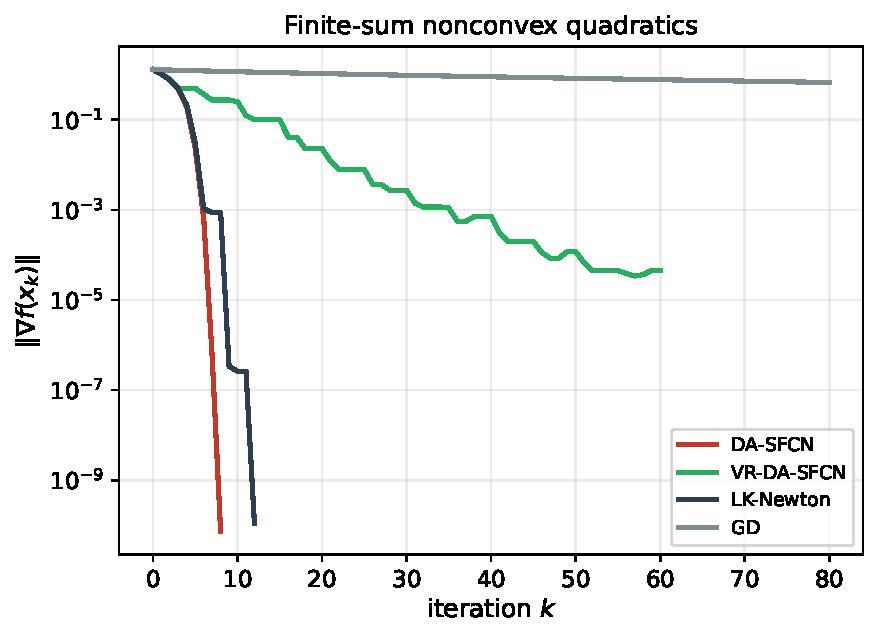
\includegraphics[width=0.48\textwidth]{fig_vr.pdf}
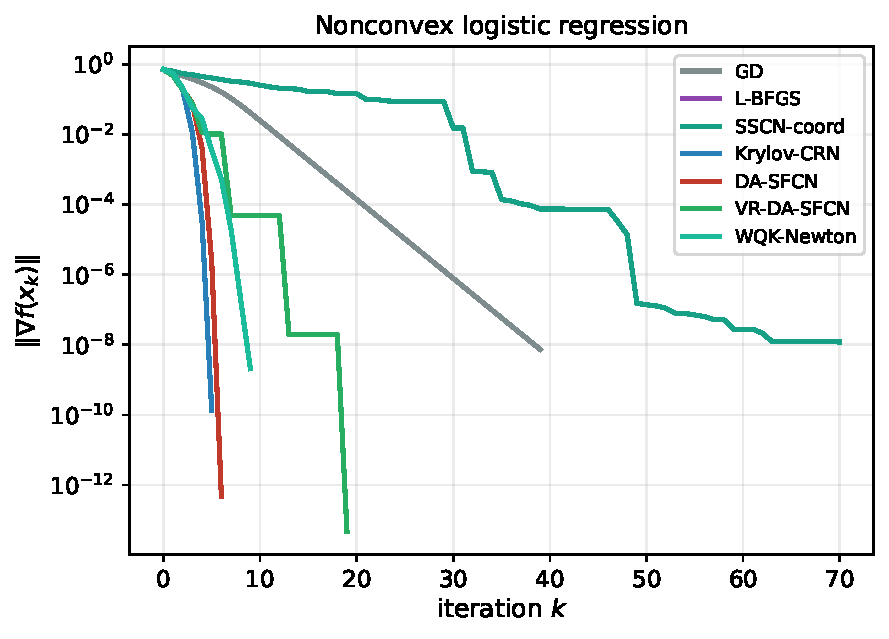
\includegraphics[width=0.48\textwidth]{fig_logistic.pdf}
\caption{يسار: 30 تربيعية غير محددة. يمين: \textenglish{VR-DA-SFCN} ضمن العائلة على اللوجستي.}
\end{figure}

\textenglish{DA-SFCN} الكامل يبلغ $7\times 10^{-11}$ في 8 خطوات؛ والمخفَّض
التباين بدمج حجم 6 يبلغ $4.6\times 10^{-5}$ في الميزانية نفسها ويواصل الهبوط.

\section{الخاتمة}
\textenglish{VR-DA-SFCN} هو حصان العمل العشوائي للعائلة: يُستخدم متى
$N\gg m_k$ وكانت لقطة التدرّج الكامل ميسورة كل $T$ خطوات.

\begin{english}
\begin{thebibliography}{9}
\bibitem{johnson2013} Johnson, Zhang. SVRG. \textit{NeurIPS}, 2013.
\bibitem{tripuraneni2018} Tripuraneni et al. \textit{NeurIPS}, 2018.
\bibitem{pasechnyuk2025} arXiv:2510.08714.
\bibitem{jiang2024} Jiang et al. \textit{AISTATS}, 2024.
\end{thebibliography}
\end{english}
\end{document}
